%\documentclass[manuscript]{aastex}

\documentclass[preprint2]{aastex}

%\documentclass[preprint]{aastex}

\newcommand{\myemail}{jluo@nrao.edu}

\slugcomment{Not to appear in Nonlearned J., 45.}

\shorttitle{GPU-accelerated pulsar search}
\shortauthors{Luo et al.}

\begin{document}

\title{Accelerating Searches for Binary Pulsars}

\author{Jintao Luo and Scott M. Ransom\altaffilmark{1}}
\affil{National Radio Astronomy Observatory, Charlottesville, VA 22903}
\email{jluo@nrao.edu}

\altaffiltext{1}{Astronomy department, University of Virginia.}


\begin{abstract}
With this paper we present our work on accelerating searches for binary pulsars 
using graphics processing units (GPUs).
The detectability of pulsars in binary systems is reduced by Doppler smearing 
due to the orbital motion. Techniques called as ``acceleration" searches have been 
developed to mitigate  this loss in sensitivity. We speed up the Fourier-domain 
acceleration search utilizing Nvidia GPUs. As the best performance, the GPU-powered 
acceleration search achieves up to $\sim$80 times speedup factor over the single-core CPU version.
\end{abstract}

\keywords{pulsar search: acceleration search: GPU: CUDA}
% test
\section{Introduction}

Pulsars are recognized as rotating neutron stars. Binary pulsars, those in 
binary systems, are of particular interest for studying relativistic physics,
 see, for example \citet{tay89}. 
Since the initial discovery of pulsars\citep{hew68}
, numerous surveys have been carried out to enlarge the number of known pulsars, 
especially binary pulsars. Searching for new pulsars is a difficult task, although it is 
conceptually simple, since it requires intensive computations.
For isolated pulsars, the search procedure includes searching the dispersion measure(DM) 
and the spin period of the pulsar. When search for a binary pulsar, there 
are additional difficulties introduced by the orbital motion.
Due to the Doppler shift, the period changes during the observation and 
the sensitivity of the search is much reduced.

Several techniques have been developed to alleviate this kind of orbital motion-caused 
sensitivity loss\citep[e.g.][]{mid84}. These so called ``acceleration'' searches operate on 
either the time domain or the frequency domain. However, extensive computing 
power is required for implementing these techniques. Generally the largest part of 
working time is spent on the process of acceleration 
search when searching for a binary pulsar.

Benefiting from Nvidia's CUDA language, we speed up the frequency-domain acceleration search 
technique developed by Scott Ransom. This acceleration is achieved by porting the program from C to CUDA C. The implementation with standard 
off-the-shelf GPUs produces a speedup factor of $\sim$80 times, as the best result, over the single-core CPU version.


\section{Acceleration Search}

\subsection{Orbital Acceleration}

The pulsed signal from a solitary pulsar with a rotation period $P_p$ can 
be represented as a sum of Fourier components:
\begin{equation}
S_p(t)=\sum_{k=1}^{\infty}a_k \exp (ik\omega_pt+i\psi_k),
\end{equation}
where $\omega_p$ = 2$\pi$$/$$P_p$ is the angular frequency of the pulsar, and 
$a_k$exp$(i\psi_k)$ is the complex amplitude of the $k$th harmonic. 
Then this signal's Fourier power spectrum, noted as $P(\omega)$, is:
\begin{equation}
P(\omega)=|\mathcal{F}[S_p(t)]|^2=|\int_{0}^{T}S_p(t)\exp (-i\omega t)dt|^2;
\end{equation}
Here $T$ is the length of the observation. 

%%$P$$(\omega)$ then consists of n spikes of height $a_k^2$ at frequency $\omega_p$, $2\omega_p$, \ldots, $n\omega_p$.

For binary pulsars, the changing velocity, as a result of the orbital motion,
 leads to a changing pulse period.
Assume the pulsar's distance to the observer $d(t)$ is changing with 
time $t$. The pulsar signal emitted at time $t$ would reach the observer 
at time $t+d(t)/c$. Here we can write the received signal $S_R(t)$ as:
\begin{equation}
S_R(t)=\sum_{k=1}^{\infty}a_k \exp \{ik\omega_p[t+d(t)/c] + i\psi_k \}.
\end{equation}
Expanding $d(t)$ in a Taylor series:
\begin{equation}
%%d(t)=d_0 + v_0t + a_0\frac{t^2}{2!} + j_0\frac{t^3}{3!}+\ldots,
d(t)=d(0) + v(0)t + a(0)\frac{t^2}{2!} + j(0)\frac{t^3}{3!}+\ldots.
\end{equation}
Here $v(t)$, $a(t)$ and $j(t)$ represent the instantaneous velocity, acceleration, and rate 
of change of acceleration respectively. Then equation $(3)$ can be rewritten as:
%where $v(t)$=$dd/dt$, $a(t)$=$d^2d/dt^2$ and $j(t)$=$d^3d/dt^3$ are the 
%instantaneous velocity, acceleration, and rate of change of acceleration, 
%respectively. Then equation $(3)$ can be rewritten as:

\begin{eqnarray}
%%\nonumber S_R(t)=\sum_{k=1}^{\infty}a_k \exp[\frac{ik\omega_pd_0}{c}]\exp[ik\omega_pt(1+\frac{v_0}{c})]\\
%%\times exp[\frac{ik\omega_pa_0t^2}{2! c}]\exp[\frac{ik\omega_pj_0t^3}{3! c}]\ldots.
\nonumber S_R(t)=\sum_{k=1}^{\infty}a_k \exp[\frac{ik\omega_pd(0)}{c}]\exp[ik\omega_pt(1+\frac{v(0)}{c})]\\
\times exp[\frac{ik\omega_pa(0)t^2}{2! c}]\exp[\frac{ik\omega_pj(0)t^3}{3! c}]\ldots.
\end{eqnarray}

%%According to this equation, $d(0)$ introduces a phase 
%%gradient $\omega_pd(0)$. This is its only contribution. 
According to this equation, the distance factor $d(0)$ only contributes by  introducing a phase shift $\omega_pd(0)$.
The velocity factor, $v(0)$, results in 
displacing harmonics from $k\omega_p$ to $k\omega_p(1+v(0)/c)$. This effect of displacement is not measurable 
since the period of a pulsar is unknown during a search.
The contribution of higher order factors is to degrade the amplitude of the harmonics 
in the power spectrum. 

When searching for binary pulsars, the signal to noise is decreased by the significant contribution from the 
acceleration factor a(0). To increase the sensitivity of the search, the acceleration-caused loss must be mitigated.


\subsection{Acceleration Search Techniques}
\citet{eat09} made a brief review on techniques commonly used in searching for binary pulsars.
A variety of so called ``acceleration'' searches have been developed to increase 
the sensitivity in searching for binary pulsars. When $T_{obs}$ $\lesssim$ 
$P_{orb}/10$, the drift of the pulsar rotating frequency caused by orbital motion 
is approximately linear hence it allows these acceleration searches to mitigate the 
loss in sensitivity almost completely. Using the recent acceleration search techniques,
binary systems with orbital periods as short as $\sim$ 90 
minutes have been discovered\citep{ran03}.
 
The direct idea to perform the acceleration search is to resample the time series, 
stretching or compressing the data to compensate for a constant frequency derivative, 
and then apply Fourier transform on the resulting series. This time-domain strategy 
is adopted by traditional acceleration searches. Another idea is to implement the
search in Fourier-domain. This method computes Fourier 
response over portions of the frequency-frequency derivative ($f-\dot{f}$) plane by
correlating a predicted Fourier response with a subset of the complex 
Fourier amplitudes in the initial full-length FFT. In this method only local Fourier amplitudes 
from an FFT of the whole dataset are used. 

Compared to their time-domain counterparts, Fourier-domain acceleration searches 
have several significant advantages:
\begin{enumerate}
  \item Fourier methods do not change the statistics of the data because they do 
not require stretching or compressing the time series while time domain methods usually
 do them using linear interpolation.
  \item The Fourier techniques use fewer FFTs as for each de-dispersed data only
one single-length FFT is required. As the contrast, the time-domain techniques 
need to perform FFT for each trial acceleration.
  \item Correlations used in the Fourier-domain search can be performed in core 
memory since only localized Fourier amplitudes are used. The fact the calculation 
is based on short FFTs and pre-computed templates allows 
efficient parallelization of Fourier-domain searches.
  \item $f-\dot{f}$ trials could be calculated independently.
\end{enumerate}


\section{Algorithm of Fourier-domain Acceleration Search}
In this section we describe the algorithm of the Fourier-domain acceleration search 
technique developed by \citet{ran02}.

Consider a signal with a normalized Fourier response of 
$A_{k-r_o}$, where $k-r_o$ is simply the frequency offset of bin $k$ from some 
reference frequency $r_o$, which goes to zero as $|k-r_o|$ approaches some 
number of bins $m/2$. The complex-valued Fourier response of such a signal at 
frequency $r_o$ can be calculated with the sum
\begin{equation}
A_{r_o}\simeq \sum_{k=[{r_o}]-m/2}^{[{r_o}]+m/2}A_k A_{r_o-k}^*
\end{equation}
If $r_o$ is initially unknown we simply compute this summation at a range of 
frequencies $r$. Calculating this equation over a range of evenly spaced 
frequencies is equivalent of correlating the raw FFT amplitude with the template 
and is therefore most efficiently computed using short FFTs and the convolution 
theorem. 

In the procedure of data process of practical pulsar searches, the raw data recorded in an observation first 
gets de-dispersed with a set of DM trials. The next step is to transform 
resulting time series into frequency domain using FFTs. To ``sweep-up'' the 
frequency range of interest, FFTs of length $M$, which is usually set to values of $1024, 
2048, \ldots, 8192$ in practical use, together with the overlap-and-save or 
overlap-and-add techniques are used to implement  correlations. 

Consider a time series $D(n)$ produced by de-dispersing the raw data with a 
certain DM, the Fourier-domain acceleration search procedure consists of following steps:
\begin{enumerate}
  \item Transform $D(n)$ into Fourier-domian with a FFT. Here we get $F(r)$.
  \item Select a range of the FFT result $F(r)$: $F_{r1}$ $-$ $F_{r2}$, 
where $r1$ and $r2$ are determined by the frequency range of interest. To correlate 
these selected frequency amplitudes via FFT-based correlations, expand them with 
a padding method to form a new series $F^{'}$.
  \item Correlate $F^{'}$ with a pre-computed template to generate a $f-\dot{f}$ 
plane.
  \item Search for candidates from the resulting $f-\dot{f}$ plane.
\end{enumerate}

\section{CUDA implementation for Fourier-domain Acceleration Search}

Using the Nvidia CUDA C language, we have implemented the Fourier-domain 
acceleration search on GPUs\footnote{Our code is available at: https://github.com/jintaoluo/presto}. As shown in figure \ref{fig:blkgram}, the implementation
computationally comprises these parts:
\begin{enumerate}
  \item Transform the data, which is the padded Fourier bins, to generate $F^{'}$ using a $M-point$ 
FFT.
	\item Transform the correlation kernels using FFTs.
  \item Time $F^{'}$ with one template plane, which is a $N\times$$M$ array 
where $N$ is the number of accelerations trials.
  \item IFFT the resulting $N\times$$M$ array and calculate its power.
  \item Do harmonic summing if necessary.
  \item Run candidates search using a specific threshold.
\end{enumerate}
The FFT/IFFT, complex-valued multiplication, power calculation, harmonic summing and 
candidate searching have been moved onto the GPU, while the reset work like candidate
 optimization are left on the CPU.
These computations involve one $M-$point FFT, $N\times$$M$ complex-valued 
multiplications and $N\times$$M$ IFFTs. If harmonic summing is needed to be done, 
array mapping and summing will occur and the number of additions will be determined by 
the number of harmonics to be summed. Candidate searching at the last step is 
relatively less computational.

%%Our code accelerates FFTs/IFFTs described in the previous 
%%section by using Nvidia's CuFFT library in the batchfft mode. Complex-valued array multiplications get parallelized as well.

%%Assume there are $N$ acceleration trials to be searched, and correlations are realized 
%%using $M-point$ FFT, conceptually in one single loop the required computations are: $N\times$$M$ complex-valued multiplications, 
%%$N$ inverse FFT and $N\times$$M$ power calculations.

\subsection{FFT and IFFT}

The time complexity of a $M-$point FFT/IFFT is 
$\mathcal{O}(M\times{\log{M}})$. If $N$ IFFTs are calculated one by one, 
the time complexity then is $\mathcal{O}(N\times{M}\times{\log{M}})$. 
The simplest way to parallelize multiple FFTs with CUDA is using Nvidia's CuFFT library in batch mode. 
In practical uses, $M$ is between 1024 and 8192, and $N$ could be as large as a few thousands. 
Assuming $M$ is 8192 and $N$ is 5000, there will be 5000 FFTs with length of 8192 to be 
calculated. The data volume then is $5000{\times}8192{\times}4=156$ MByte. This can be easily 
fit to modern GPUs, which are usually equipped with more than 2 GByte on-chip memories.

In concept, it is required to Fourier transform the templates to implement FFT-based correlations. Since the 
resulting planes are reusable, they can be stored as constant coefficients after being pre-calculated. Then significant
 computing resources get saved by avoiding calculating these planes repeatedly. 
 
\subsection{Complex-valued Multiplication}
$F^{'}$ times the template plane's $N$ rows and multiplications are done point-to-point.
These complex-valued multiplications are independent from each other, then can be carried out in  
parallel on GPUs. The use of GPU's texture memory helps enhance the performance. If the template 
plane's size is relatively small, it can be bound to the texture memory together with $F^{'}$ to  
improve the read access to their contents.

\subsection{Power Calculation}
Powers of results from the correlation are calculated for the following candidate searching operation. A part  
of a FFT-based correlation's output need to be discarded or ``chopped'' because they are not valid products.
So computing power then can be saved by only carrying out power calculations on the valid correlation output. 
 
Like complex-valued multiplications, power calculations are applied to each single data point
individually. That means it could benefit from the GPU's intrinsic parallelization capability as well.

\subsection{Harmonic Summing}

Duty cycles of pulsar signals generally range between 1\% and 50\%\citep{joh91},
 resulting between 1 and 50 harmonics in their power spectrums. Taking advantage of 
this fact, ``harmonic summing'' of the power spectrum of the 
de-dispersed time series is utilized to increase the sensitivity in searches. 

To do harmonic summing, conceptually, the power in the Fourier transform at frequencies
$2f$, $3f$, \ldots, $nf$ are summed with the one at frequency $1f$.
Taking  $\dot{f}$ into consideration, harmonic summing then becomes
to add a harmonic's $f-\dot{f}$ plane to the fundamental plane. 
The amount of harmonics to sum up is determined by the input parameter $numharm$. 
Generally, he harmonic plane's size is smaller and needs to be scaled to the size of the fundamental one. In 
our implementation, the scale-up is realized by using a mapping method. To save computing resources, mapping
indexes are pre-calculated with CPU and then stored on GPU. Additions are computed in parallel since each point 
in the fundamental plane gets added with only one point from the hramonic plane. 

2D texture memory is used to improve data accesses to scale-up indexes and
harmonic planes. Access to GPU's global memory, in which the on-GPU data is stored by default, is relatively
time consuming. To minimize the number of 
this kind of access, harmonic summing is carried out together with the power calculation. If a point in the
harmonic plane is usable, which means it will be used for power calculation and then harmonic summing, it 
will be read out only once. The following computations, power calculation and adding, will be placed in the same 
thread to save time.

\subsection{Candidate Searching}
The candidate searching follows harmonic summing to check
the summed powers with a threshold.  
The qualified candidates, whose values are larger than the threshold, will be stored in the GPU's global memory and 
transfered back to the CPU later. The stored content includes not only the data value, but also other information like
the corresponding frequency. This operation benefits from the use of texture memory as well.
Like aforementioned power calculation, comparisons in candidate searching are done on each point independently. So they 
can be carried out in parallel. However counting the total number
of qualified candidates should be done carefully, since it is likely multiple qualified candidates would request to modify
the counter simultaneously. This risk is avoided via using a lock strategy realized with the use of atomic CUDA addition.

\section{Results}
The Fourier-domain acceleration search technique developed by Scott Ransom was realized as a program within
PRESTO(PulsaR Exploration and Search TOolkit) which is a large suite of pulsar search and analysis software.
Instead of creating a new individual program,
our GPU-powered acceleration search code was developed as a patch or expansion to the original CPU-only program.

To test the code, files containing pulsed signals was generated using fake pulsar generator within PRESTO.
Additionally, data recorded in real observations were used as well. Details of the three machines 
used to carry out these tests are listed in table \ref{tbl-machine}. 
And we have some cooperators help test the code with their own data and machines.

\subsection{Fake data}
Table \ref{tbl-simupara} lists parameters which were used to generate fake data files. These files were 
generated as time series with different amounts of data points.

Figure \ref{fig:runtime} shows the performance on machine {\#}1 when processing fake files. A Nvidia GTX 780 GPU
was used to run the CUDA implementation code. And one of the 12 cores in a 3.20 GHz Intel Xeon 
E5-1650 CPU was used to do the CPU implementation. For both implementations, as shown in igure \ref{fig:runtime},
the general tendency is for total runtime to increase linearly as the number of data points increases. 
The parameter $zmax$ was set to 256, and values of $numharm$ are given in the figure's description.

Benchmarks on machines previously introduced are used to produce plots in figure \ref{fig:numharm_effect}. 
On each machine, the GPU did the acceleration search on a group of fake files, with $zmax$ set to 256 and 
$numharm$ assigned as 1 and 16. The CPU's performance is used to calculate speedup factors.

As figure \ref{fig:numharm_effect} shows, most benchmarks using 1 harmonics produce larger
speedup factors than their 16-harmonic counterparts. Among results from machine {\#}2 there are two exceptions.
And there is one exception in results from machine {\#}3. The smaller $numharm$ means fewer 
harmonic summing operations. When this parameter is set to 1, there is completely no harmonic summing
to be done. The fact that smaller $numharm$ produces better speedup factor suggests that optimizing the on-GPU harmonic 
summing could lead to further improvement to our CUDA implementation.

\subsection{Real data}
Data from an observation on Terzan5 using GBT was used as real data to test the GPU-powered acceleration search code. The 
observation was made on Jul. 5, 2012, with a total bandwidth of 800 MHz centering round the frequency of 1105 MHz. 
A DM value of 239.93
was used to de-disperse the search mode raw data. The de-dispersion produced files with various lengths of data points. 
The sampling time in resulting files is 40.96 $\mu$s.

Tests were carried out with machine {\#}1. The parameter $numharm$ was set to 8, and $zmax$ was assigned values 
5, 20, 50, 200, and 500. As shown in figure \ref{fig:Terzan5_8_harm}, larger $zmax$ results in higher speedup. 
And similar to curves in figure \ref{fig:numharm_effect}.(a), which represents results on machine {\#}1 processing fake data, 
speedup factors increase as the number of data points increases. However in figure \ref{fig:Terzan5_8_harm} the curve 
for 500-$zmax$ does not strictly follow this tendency, having less data point produces better speedup factor. 
This might be due to the noise level fluctuations in the raw data, 
which results in different noise levels in dedispersed files
with different lengths.

\section{Conclusions and Discussions}
We have implemented a Fourier-domain acceleration search technique on GPUs using CUDA. This has led to a 
GPU-over-CPU performance speedup, which varies depending on parameter configurations and GPUs and CPUs 
that are used, of up to ~80x. 

Conclusions can be made from benchmarks on simulation and real data files:
\begin{enumerate}
  \item Generally the larger data length produces larger GPU-on-CPU speedup factor.
  \item Larger $zmax$ would cause higher speedup factor.
  \item Smaller $numharm$ responds to larger speedup factor.
\end{enumerate}

The explanation to $zmax$'s effect is there are more FFTs to be done when $zmax$ is larger. And GPUs work pretty well in 
accelerating FFT computations. So the more FFTs, the larger speedup factor.

The reason why smaller $numharm$, not the larger one, produces the higher speedup factor is the on-GPU 
implementation for harmonic summing is not as good as for FFTs which utilize Nvdia's cuFFT library. 

Work is ongoing with plans to maximize the usage of GPUs by using multithread technique. It is 
expected the current performance can be doubled. 
\section{Acknowledgments}
This work is supported by the NSF PIRE award.

\begin{figure}
\centering
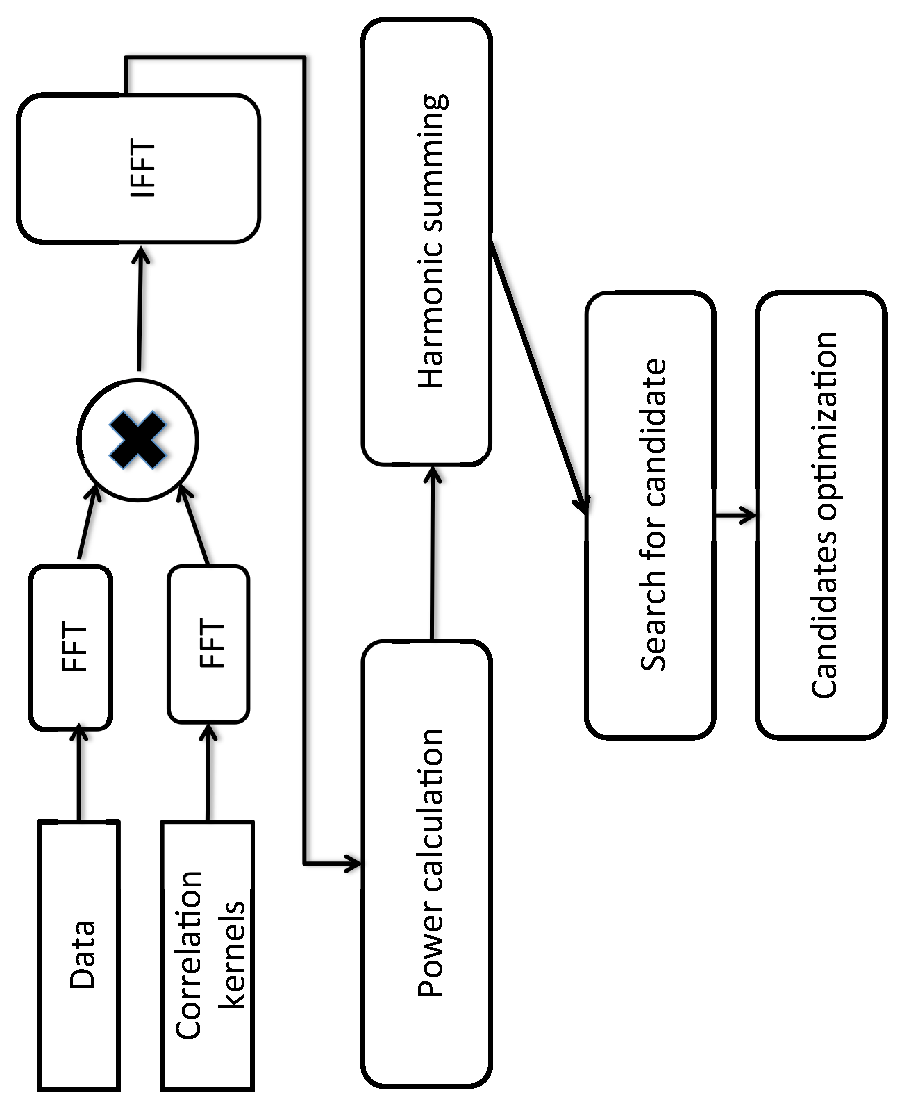
\includegraphics[angle=-90, width=0.5\textwidth]{fig/accelsearch_diagram.eps}
\caption{The block diagram of Fourier-domain acceleration search.}
\label{fig:blkgram}
\end{figure}

\begin{figure}
  \centering
  \begin{tabular}[b]{@{}p{0.50\textwidth}@{}}
    \centering\includegraphics[width=1.0\linewidth]{fig/makalu_runtime_overview_1_harm.eps} \\
    \centering\small (a) 1 harmonic
  \end{tabular}%
  \quad
  \begin{tabular}[b]{@{}p{0.50\textwidth}@{}}
    \centering\includegraphics[width=1.0\linewidth]{fig/makalu_runtime_overview_16_harm.eps} \\
    \centering\small (b) 16 harmonics
  \end{tabular}
\caption{Run time on makalu machine, with different harmonics.}
\label{fig:runtime}
\end{figure}


\begin{figure}
  \centering
  \begin{tabular}[b]{@{}p{0.50\textwidth}@{}}
    \centering\includegraphics[width=1.0\linewidth]{fig/makalu_speed_up.eps} \\
    \centering\small (a) makalu
  \end{tabular}%
  \quad
  \begin{tabular}[b]{@{}p{0.50\textwidth}@{}}
    \centering\includegraphics[width=1.0\linewidth]{fig/zuul05_speed_up.eps} \\
    \centering\small (b) zuul05
  \end{tabular}
  \quad
  \begin{tabular}[b]{@{}p{0.50\textwidth}@{}}
    \centering\includegraphics[width=1.0\linewidth]{fig/sh_machine_speed_up.eps} \\
    \centering\small (b) sh machine
  \end{tabular}
\caption{Speed-up factors: GPU on CPU.}
\label{fig:numharm_effect}
\end{figure}

\begin{figure}
\centering
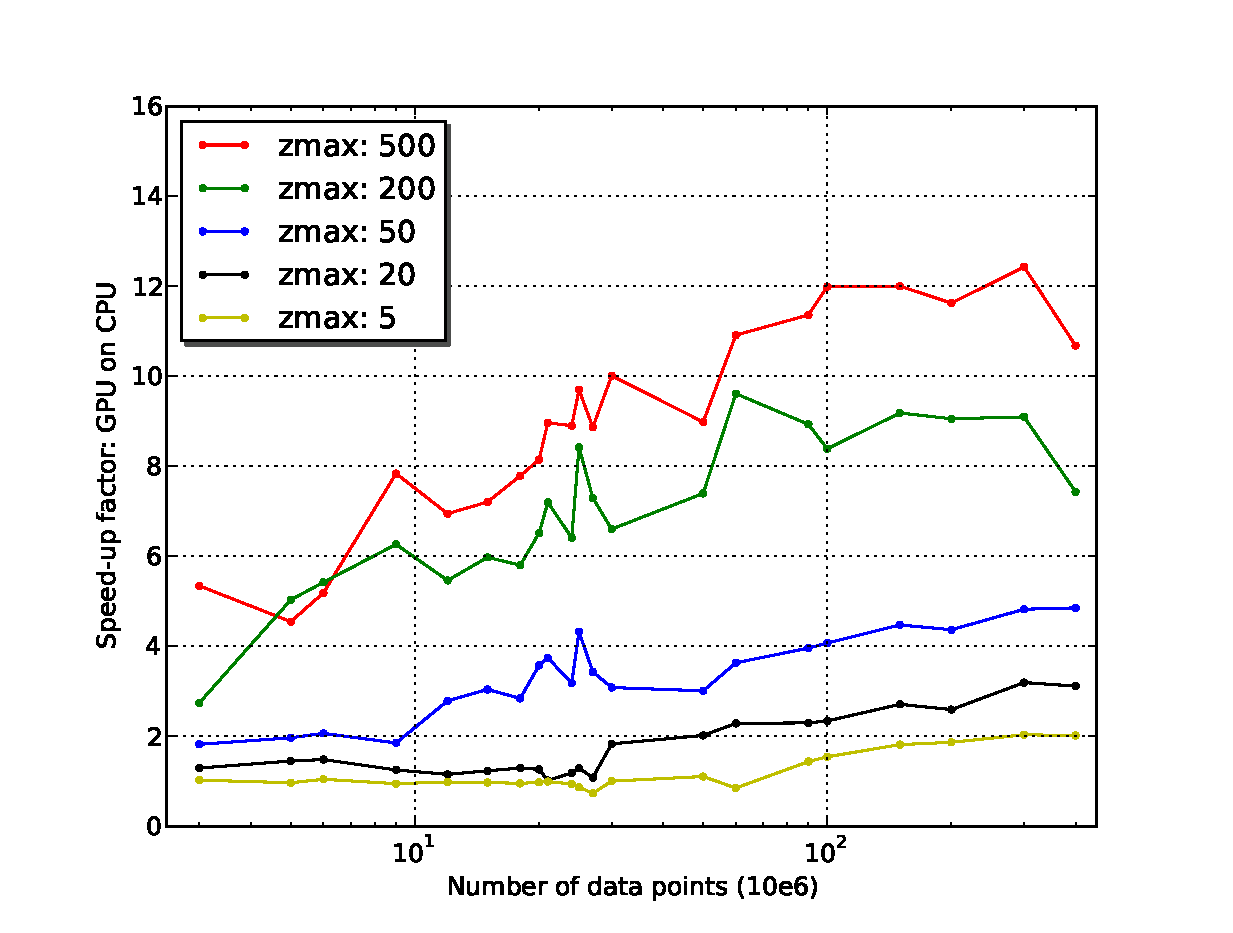
\includegraphics[width=0.5\textwidth]{fig/Terzan5_s000m_8_harm_makalu.eps}
\caption{Benchmarks on real observation data.}
\label{fig:Terzan5_8_harm}
\end{figure}

%\begin{figure}
%\plotone{fig/Terzan5_s000m_8_harm_makalu.eps} \\    
%\caption{Benchmarks on real observation data.}
%\label{fig:Terzan5_8_harm}
%\end{figure}

\begin{table}
\begin{center}
\caption{Platforms Used in Investigations. \label{tbl-machine}}
\begin{tabular}{cccc}
\tableline\tableline
Machine & GPU & CPU & System Memory \\
\tableline
1 & Nvidia Geforce GTX 780 & Intel Xeon E5-1650 & 62 GByte\\
2 & Nvidia Geforce GTX 780 & Intel Xeon E5-2640 & 63 GByte\\
3 & Nvidia Geforce GTX Titan & Intel Xeon E5-2670 & 126 GByte
\end{tabular}
\end{center}
\end{table}

\begin{table}
\begin{center}
\caption{Parameters used to generate fake file. \label{tbl-simupara}}
\begin{tabular}{lc}
\tableline\tableline
Parameter & Value\\
\tableline
Sample time & 64 $\mu$s\\
Pulse Frequency($f$) & 123.876876786 Hz\\
$\dot{f}$ & 1.123e-6 $s^{-2}$\\
Noise Sigma & 14.142135623731
\end{tabular}
\end{center}
\end{table}



\begin{thebibliography}{}

\bibitem[Eatough(2009)]{eat09}Eatough, R. H. 2009, \ PhD thesis, University of 
Manchester

%\bibitem[Hamilton, Helfand, and Becker(1985)]{ham85}Hamilton, T. T., Helfand, D. 
%J., \& Becker, R. H. 1985, AJ, 90, 606

\bibitem[Hewish et al.(1968)]{hew68}Hewish, A., Bell, S. J., Pilkington, J. D. 
H., Scott, P. F., \& Collins, R. A.  1968,Nature, 217, 709

\bibitem[Johnston \& Kulkarni(1991)]{joh91}Johnston, H. M., \& Kulkarni, S. M.  
1991, AJ, 368, 504

\bibitem[Kulkarni \& Anderson(1996) ]{kul96}Kulkarni, S. R., \& Anderson, S. B. 
1996, in IAU Symp. 174, Dynamical Evolution of Star Clusters: Confrontation of 
Theory and Observations, ed. P. Hut \& J. Makino (Dordrecht: Kluwer), 181 

\bibitem[Lyne(1995)]{lyn95}Lyne, A. G. 1995, in ASP Conf. Ser. 72, Millisecond 
Pulsars: A Decade of Surprise, ed. A. S. Fruchter, M. Tavani, \& D. C. Backer 
(San Francisco: ASP), 35

\bibitem[Middleditch \& Kristian(1984)]{mid84}Middleditch, J., \& Kristian, J.  
1984, ApJ, 279, 157

\bibitem[Ransom et al.(2002)]{ran02}Ransom, S. M., Eikenberry, S. S., \& Middleditch,
 J. 2002, AJ, 124, 1788

\bibitem[Ransom et al.(2003)]{ran03}Ransom, S. M., Cordes, J. M., \& Eikenberry, S. S. 
2003,  ApJ, 589, 911

\bibitem[Taylor \& Weisberg(1982)]{tay89}Taylot, J.H., Weisberg, J.M. 1989, ApJ, 345, 434

%\bibitem[Ransom(2001)]{ran01}Ransom, S. M. 2001,\ PhD thesis, Harvard University

\end{thebibliography}


\end{document}
